\documentclass[11pt,a4paper]{article}
\usepackage[utf8]{inputenc}
\usepackage[vietnamese]{babel}
\usepackage{amsmath,amssymb}
\usepackage[version=4]{mhchem}
\usepackage{geometry}
\geometry{top=1.5cm,bottom=1.2cm,left=1.4cm,right=1.4cm,headheight=28pt,headsep=12pt,footskip=18pt}
\usepackage{graphicx}
\usepackage{xcolor}
\usepackage{tabularx}
\usepackage{array}
\usepackage{tikz}
\usepackage{multicol}
\usepackage{fancyhdr}
\usepackage{enumitem}

\definecolor{hfRed}{HTML}{D32F2F}
\definecolor{hfGreen}{HTML}{8BC390}
\definecolor{mainGreen}{HTML}{2E7D32}

\usepackage{ex_test}

\pagestyle{fancy}
\fancyhf{}
\renewcommand{\headrulewidth}{0.75pt}
\renewcommand{\headrule}{\hbox to\headwidth{\color{hfGreen}\leaders\hrule height \headrulewidth\hfill}}
\renewcommand{\footrulewidth}{0.75pt}
\renewcommand{\footrule}{\hbox to\headwidth{\color{hfGreen}\leaders\hrule height \footrulewidth\hfill}}

\fancyhead[L]{\small\itshape\color{hfRed}Tài liệu lưu hành nội bộ}
\fancyhead[R]{\small\color{hfRed}Thầy \textbf{TRẦN VĂN THẠNH} - 0777.470.803}

\fancyfoot[L]{\footnotesize\itshape\color{hfRed}CS1: 6/15 Nguyễn Hoàng, P. Kim Long, TP Huế \quad|\quad CS2: 24 Đặng Thái Thân, TP Huế}
\fancyfoot[R]{\small\textbf{\color{hfRed}Trang \thepage}}

\setlength{\parindent}{0pt}
\setlength{\parskip}{1.4pt}

\def\loigiai#1{
\par\begingroup\color{blue!80!black}\small
\noindent\textbf{\textit{Lời giải chi tiết:}}\par
#1\par\endgroup}

\begin{document}

\Opensolutionfile{ans}[ans-de11-gv]

\noindent
\begin{minipage}[t]{0.48\textwidth}
	\centering
	\textbf{SỞ GIÁO DỤC VÀ ĐÀO TẠO THỪA THIÊN HUẾ}\\
	\textbf{TRƯỜNG THPT HAI BÀ TRƯNG}\\
	\textbf{ĐỀ CHÍNH THỨC}\\
	\textit{(Đề thi có 04 trang)}
\end{minipage}\hfill
\begin{minipage}[t]{0.48\textwidth}
	\centering
	\textbf{\color{mainGreen}ĐỀ KIỂM TRA ĐỊNH KỲ CHƯƠNG 4 (POLYMER)}\\
	\textbf{MÔN: HOÁ HỌC -- LỚP 12}\\
	\textit{Thời gian làm bài: 50 phút (không kể thời gian phát đề)}\\
	\textbf{Mã đề thi: 111}
\end{minipage}


\vspace{0.1cm}
\begin{center}
	\textbf{\color{hfRed}\Large (BẢN GIÁO VIÊN -- CÓ LỜI GIẢI CHI TIẾT)}
\end{center}

\vspace{0.1cm}
\noindent\textit{Họ, tên thí sinh: \dots\dots\dots\dots\dots\dots\dots\dots\dots\dots\dots\dots\dots\dots\dots\dots\dots\dots\dots\dots\dots\dots Lớp: \dots\dots\dots\dots SBD: \dots\dots\dots\dots}\\
\noindent\textit{(Cho biết nguyên tử khối: H = 1; C = 12; N = 14; O = 16; Na = 23; Al = 27; S = 32; Cl = 35,5; K = 39; Ca = 40; Fe = 56; Cu = 64; Zn = 65; Br = 80; Ag = 108; Ba = 137).}

\vspace{0.15cm}
\noindent
\textbf{PHẦN I (4,5 điểm -- 18 câu): Câu trắc nghiệm nhiều phương án lựa chọn.}\\
\textit{Thí sinh trả lời từ câu 1 đến câu 18. Mỗi câu hỏi thí sinh chỉ chọn một phương án.}

\setcounter{ex}{0}

\begin{ex}
(SBT -- KNTT). Chất nào dưới đây thuộc loại polymer?
\choice
{Glucose}
{Fructose}
{Saccharose}
{\True Cellulose}
\loigiai{
Cellulose là polysaccharide có công thức phân tử là \ce{(C6H10O5)_n} ($n \approx 1000 - 14000$) thuộc loại polymer thiên nhiên. Glucose và fructose là monosaccharide; saccharose là disaccharide.\\
\textbf{Chọn D.}}
\end{ex}

\begin{ex}
(SBT -- KNTT). Tính chất vật lí chung của polymer là
\choice
{chất lỏng, không màu, không tan trong nước}
{chất lỏng, không màu, tan tốt trong nước}
{chất rắn, không bay hơi, dễ tan trong nước}
{\True chất rắn, không bay hơi, không tan trong nước}
\loigiai{
Hầu hết các polymer ở nhiệt độ thường là chất rắn, không bay hơi, không tan trong nước và không có nhiệt độ nóng chảy xác định.\\
\textbf{Chọn D.}}
\end{ex}

\begin{ex}
Polymer nào sau đây bị thủy phân trong dung dịch \ce{NaOH}?
\choice
{\True Poly(vinyl acetate)}
{Polyethylene}
{Polypropylene}
{Polybuta-1,3-diene}
\loigiai{
Poly(vinyl acetate) (PVAc) có chứa nhóm chức ester trong mạch nhánh \ce{[-CH2-CH(OCOCH3)-]_n}, khi đun nóng với dung dịch kiềm sẽ bị thủy phân tạo poly(vinyl alcohol) và muối acetate. Các polymer còn lại chỉ có liên kết carbon--carbon bền vững nên không bị thủy phân.\\
\textbf{Chọn A.}}
\end{ex}

\begin{ex}
Polymer nào sau đây có thể bị thuỷ phân hoàn toàn trong môi trường acid hoặc môi trường base thu được amino acid?
\choice
{Tinh bột}
{\True Tơ capron}
{Polypropylene}
{Poly(vinyl chloride)}
\loigiai{
Tơ capron (polycaproamide) có chứa liên kết amide \ce{-CO-NH-}: \ce{[-NH-(CH2)5-CO-]_n}, khi thủy phân hoàn toàn trong môi trường acid hoặc base sẽ tạo ra $\varepsilon$-aminocaproic acid (\ce{H2N-(CH2)5-COOH}) hoặc muối tương ứng. Tinh bột thủy phân tạo glucose; PP và PVC không bị thủy phân.\\
\textbf{Chọn B.}}
\end{ex}

\begin{ex}
(SBT -- KNTT). Trên hộp xốp cách nhiệt, hộp đựng thức ăn mang về, cốc, chén đĩa dùng một lần,\dots{} thường được in kí hiệu như hình bên. Polymer dùng làm các đồ dùng đó được tổng hợp từ monomer nào sau đây?
\begin{center}
	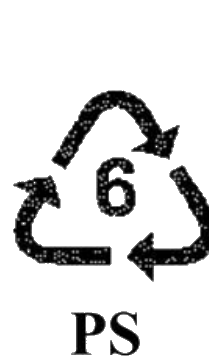
\includegraphics[width=1.5cm]{images_crop_de11/cau5_ps_symbol.png}
\end{center}
\choice
{\ce{CH2=CH2}}
{\ce{CH2=CH-CH3}}
{\True \ce{CH2=CH-C6H5}}
{\ce{CH2=CHCl}}
\loigiai{
Kí hiệu số 6 cùng chữ PS là mã nhận diện của polystyrene. Polystyrene được điều chế bằng phản ứng trùng hợp styrene (vinylbenzene, \ce{CH2=CH-C6H5}).\\
\textbf{Chọn C.}}
\end{ex}

\begin{ex}
(SBT -- KNTT). Phân tử polymer nào sau đây chỉ chứa hai loại nguyên tố?
\choice
{Poly(methyl methacrylate)}
{Poly(vinyl chloride)}
{Polyacrylonitrile}
{\True Polypropylene}
\loigiai{
Polypropylene (PP) có công thức là \ce{[-CH2-CH(CH3)-]_n} chỉ chứa 2 nguyên tố C và H. Poly(methyl methacrylate) chứa C, H, O; PVC chứa C, H, Cl; polyacrylonitrile chứa C, H, N.\\
\textbf{Chọn D.}}
\end{ex}

\begin{ex}
(SBT -- KNTT). Tơ tằm, sợi bông, len thuộc loại tơ nào sau đây?
\choice
{\True Tơ tự nhiên}
{Tơ tổng hợp}
{Tơ bán tổng hợp}
{Tơ nhân tạo}
\loigiai{
Tơ tằm, sợi bông, len lông cừu là các loại tơ có sẵn trong tự nhiên từ động vật hoặc thực vật nên thuộc loại tơ tự nhiên (tơ thiên nhiên).\\
\textbf{Chọn A.}}
\end{ex}

\begin{ex}
(SBT -- KNTT). Tơ nào sau đây thuộc loại tơ bán tổng hợp?
\choice
{Tơ nylon-6,6}
{\True Tơ cellulose acetate}
{Tơ capron}
{Tơ tằm}
\loigiai{
Tơ cellulose acetate và tơ visco là tơ bán tổng hợp (tơ nhân tạo) được chế tạo bằng cách biến đổi hóa học polymer thiên nhiên (cellulose). Tơ nylon-6,6 và tơ capron là tơ tổng hợp; tơ tằm là tơ tự nhiên.\\
\textbf{Chọn B.}}
\end{ex}

\begin{ex}
(SBT -- KNTT). Polymer nào sau đây \textbf{không} thuộc loại cao su?
\choice
{\True Poly(methyl methacrylate)}
{Polychloroprene}
{Polyisoprene}
{Polybuta-1,3-diene}
\loigiai{
Poly(methyl methacrylate) là chất dẻo (thủy tinh hữu cơ plexiglass). Ba chất còn lại đều là các loại cao su.\\
\textbf{Chọn A.}}
\end{ex}

\begin{ex}
Cho các polymer: polyethylene, tơ nitron, tơ capron, nylon-6,6, tinh bột, protein, cao su isoprene và cao su buna-N. Số polymer có chứa nitrogen trong phân tử là
\choice
{\True 5}
{6}
{7}
{4}
\loigiai{
Các polymer chứa nitrogen gồm 5 chất: tơ nitron (\ce{[-CH2-CH(CN)-]_n}), tơ capron (\ce{[-NH-(CH2)5-CO-]_n}), nylon-6,6 (\ce{[-NH-(CH2)6-NH-CO-(CH2)4-CO-]_n}), protein (chuỗi polypeptide chứa N), cao su buna-N (đồng trùng hợp buta-1,3-diene và acrylonitrile, chứa N).\\
\textbf{Chọn A.}}
\end{ex}



\begin{ex}
Cho các polymer sau: cellulose, amylose, amylopectin, poly(ethylene terephthalate), polybuta-1,3-diene, polyisoprene. Số polymer thiên nhiên là
\choice
{5}
{2}
{3}
{\True 4}
\loigiai{
Các polymer thiên nhiên gồm 4 chất: cellulose, amylose, amylopectin, polyisoprene (thành phần chính trong mủ cây cao su thiên nhiên). PET và polybuta-1,3-diene là polymer tổng hợp.\\
\textbf{Chọn D.}}
\end{ex}

\begin{ex}
Có một số hợp chất sau: (1) ethylene, (2) vinyl chloride, (3) adipic acid, (4) phenol, (5) acrylonitrile, (6) buta-1,3-diene. Những chất nào có thể tham gia phản ứng trùng hợp?
\choice
{\True (1), (2), (5), (6)}
{(1), (2), (3), (4)}
{(1), (4), (5), (6)}
{(2), (3), (4), (5)}
\loigiai{
Các monomer tham gia phản ứng trùng hợp phải chứa liên kết đôi \ce{C=C} hoặc vòng kém bền: (1) \ce{CH2=CH2}, (2) \ce{CH2=CHCl}, (5) \ce{CH2=CH-CN}, (6) \ce{CH2=CH-CH=CH2}. Adipic acid và phenol chỉ tham gia phản ứng trùng ngưng.\\
\textbf{Chọn A.}}
\end{ex}

\begin{ex}
Dãy nào sau đây đều thuộc loại polymer tổng hợp?
\choice
{\True Tơ capron, tơ nitron, cao su buna}
{Polystyrene, tơ tằm, tơ nylon-6,6}
{Tơ cellulose acetate, cao su buna-S, tơ nylon-6}
{Tơ viscose, tơ olon, tơ nylon-7}
\loigiai{
Tơ capron, tơ nitron, cao su buna đều là các polymer được tổng hợp nhân tạo từ monomer đơn giản. Phương án B có tơ tằm (thiên nhiên); C và D chứa tơ cellulose acetate, tơ viscose (bán tổng hợp).\\
\textbf{Chọn A.}}
\end{ex}

\begin{ex}
Cho các polymer sau: polybuta-1,3-diene, poly(methyl methacrylate), polyacrylonitrile, nylon-6,6. Số polymer được điều chế bằng phản ứng trùng ngưng là
\choice
{3}
{2}
{4}
{\True 1}
\loigiai{
Chỉ có 1 polymer được điều chế bằng phản ứng trùng ngưng là nylon-6,6 (trùng ngưng hexamethylenediamine và adipic acid). Ba polymer còn lại được điều chế bằng phản ứng trùng hợp.\\
\textbf{Chọn D.}}
\end{ex}

\begin{ex}
Phát biểu nào sau đây sai?
\choice
{\True Trùng ngưng buta-1,3-diene thu được polymer dùng để sản xuất chất dẻo}
{Trùng hợp ethylene thu được polymer dùng để sản xuất chất dẻo}
{Trùng ngưng $\varepsilon$-aminocaproic acid thu được polycaproamide}
{Trùng hợp vinyl cyanide thu được polymer dùng để sản xuất tơ nitron (tơ olon)}
\loigiai{
Phát biểu A sai vì buta-1,3-diene tham gia phản ứng \textbf{trùng hợp} (không phải trùng ngưng) và sản phẩm là polybutadiene dùng sản xuất \textbf{cao su buna} (không phải chất dẻo).\\
\textbf{Chọn A.}}
\end{ex}

\begin{ex}
Không nên ủi (là) quá nóng quần áo bằng nylon, len, tơ tằm vì
\choice
{\True len, tơ tằm, tơ nylon có các nhóm liên kết trong phân tử kém bền với nhiệt}
{len, tơ tằm, tơ nylon mềm mại}
{len, tơ tằm, tơ nylon là những sợi thấm nước}
{len, tơ tằm, tơ nylon không thể là phẳng}
\loigiai{
Len lông cừu, tơ tằm (protein) và tơ nylon (polyamide) đều chứa các liên kết amide/peptide \ce{-CO-NH-} kém bền nhiệt, ở nhiệt độ cao các liên kết này dễ bị đứt gãy làm sợi vải co rúm, giòn và hỏng.\\
\textbf{Chọn A.}}
\end{ex}

\begin{ex}
(SBT -- CTST). Khối lượng của một đoạn mạch nylon-6,6 là 27 346 amu và của một đoạn mạch capron (nylon-6) là 17 176 amu. Số lượng mắt xích trong đoạn mạch nylon-6,6 và capron nêu trên lần lượt là
\choice
{113 và 152}
{121 và 114}
{\True 121 và 152}
{113 và 114}
\loigiai{
- Mắt xích nylon-6,6 có công thức \ce{[-NH-(CH2)6-NH-CO-(CH2)4-CO-]} với $M = 226\text{ amu}$.\\
Số mắt xích trong đoạn mạch nylon-6,6:
$$n = \frac{27346}{226} = 121.$$
- Mắt xích capron có công thức \ce{[-NH-(CH2)5-CO-]} với $M = 113\text{ amu}$.\\
Số mắt xích trong đoạn mạch capron:
$$n = \frac{17176}{113} = 152.$$
\textbf{Chọn C.}}
\end{ex}

\begin{ex}
Tơ là những vật liệu polymer hình sợi dài và mảnh với độ bền nhất định. Cho các phát biểu sau về tơ:\\
(a) Mạch phân nhánh, xếp song song với nhau.\\
(b) Mềm, dai, không độc, tương đối bền với các dung môi thông thường và có khả năng nhuộm màu.\\
(c) Nguyên liệu quan trọng trong ngành luyện kim.\\
(d) Tơ tự nhiên: Là tơ có sẵn trong thiên nhiên như bông, sợi lanh, len lông cừu, tơ tằm,\dots\\
(e) Tơ tổng hợp: Là tơ được chế tạo từ polymer tổng hợp như polyamide (nylon, capron,\dots).\\
(f) Tơ bán tổng hợp: Là tơ xuất phát từ nguồn thiên nhiên nhưng được chế biến thêm bằng phương pháp hoá học (như tơ visco, tơ cellulose acetate,\dots).\\
Số phát biểu đúng là
\choice
{6}
{3}
{5}
{\True 4}
\loigiai{
Các phát biểu đúng là: (b), (d), (e), (f) (gồm 4 phát biểu).\\
- (a) Sai vì tơ có cấu trúc mạch \textbf{không phân nhánh}.\\
- (c) Sai vì tơ là nguyên liệu quan trọng của ngành \textbf{dệt may}.\\
\textbf{Chọn D.}}
\end{ex}



\noindent
\textbf{PHẦN II (4,0 điểm -- 4 câu): Câu trắc nghiệm đúng sai.}\\
\textit{Thí sinh trả lời từ câu 1 đến câu 4. Trong mỗi ý a), b), c), d) ở mỗi câu, thí sinh chọn đúng hoặc sai.}

\setcounter{ex}{0}

\begin{ex}
(SBT -- KNTT). Polymer X có thể chịu được nhiệt độ lên tới 160 $^\circ\text{C}$ nên được dùng làm ống dẫn nước nóng, hộp đựng thực phẩm có thể sử dụng trong lò vi sóng,\dots{} Các vật dụng làm từ X thường được in kí hiệu như hình bên.
\begin{center}
	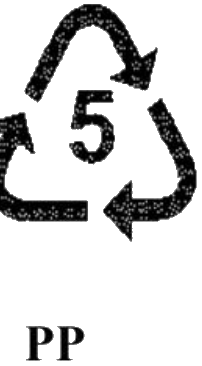
\includegraphics[width=1.5cm]{images_crop_de11/p2_cau1_pp_symbol.png}
\end{center}
\choiceTF
{X được tổng hợp từ phản ứng trùng hợp pent-1-ene}
{\True Hộp nhựa làm từ X có thể đựng nước sôi mà không bị biến dạng}
{\True X thuộc loại polymer nhiệt dẻo}
{\True Nhựa làm từ X thuộc loại nhựa có thể tái chế}
\loigiai{
a) \textbf{Sai}. Polymer X là polypropylene (PP), được điều chế bằng phản ứng trùng hợp propylene (propene, \ce{CH2=CH-CH3}).\\
b) \textbf{Đúng}. PP chịu được nhiệt độ lên tới 160 $^\circ\text{C}$, cao hơn nhiệt độ sôi của nước (100 $^\circ\text{C}$) nên đựng được nước sôi mà không biến dạng.\\
c) \textbf{Đúng}. PP là polymer nhiệt dẻo, nóng chảy khi đun nóng và đông cứng khi để nguội.\\
d) \textbf{Đúng}. Kí hiệu số 5 PP thuộc hệ thống các loại nhựa có thể thu gom và tái chế.}
\end{ex}

\begin{ex}
(SBT -- CĐ). Tơ visco được sản xuất phổ biến từ đầu thế kỉ XX, là một loại chất liệu được làm từ bột gỗ của cây như tre, đậu nành, mía,\dots, qua quá trình xử lí hoá học được sợi visco. Sợi visco thấm hút mồ hôi và thoáng khí, mềm mại nên rất phổ biến trong việc sản xuất quần áo, đặc biệt là trang phục mùa hè vì nó giúp người mặc cảm thấy mát mẻ và thoải mái. Những phát biểu nào sau đây là đúng?
\choiceTF
{Tơ visco thuộc loại tơ thiên nhiên}
{\True Tơ visco thuộc loại tơ bán tổng hợp}
{\True Sợi visco có thành phần chính là cellulose đã được xử lí hoá chất}
{\True Tơ là vật liệu polymer hình sợi, dài, mảnh, có độ bền nhất định, mạch không nhánh}
\loigiai{
a) \textbf{Sai}. Tơ visco thuộc loại tơ bán tổng hợp (tơ nhân tạo).\\
b) \textbf{Đúng}. Sợi visco có nguồn gốc từ thiên nhiên (gỗ) nhưng được chế biến bằng hóa chất.\\
c) \textbf{Đúng}. Cellulose từ bột gỗ được xử lí với \ce{CS2} và dung dịch \ce{NaOH} tạo chất keo nhớt visco, sau đó ép vào bể acid tái sinh sợi cellulose.\\
d) \textbf{Đúng}. Đây là các đặc tính vật lí và cấu trúc phân tử cơ bản của vật liệu tơ sợi.}
\end{ex}

\begin{ex}
(SBT -- CĐ). Keo dán dùng để kết dính các vật liệu và được sử dụng rộng rãi trong đời sống, sản xuất. Những phát biểu nào sau đây là đúng?
\choiceTF
{\True Nhựa vá săm là dung dịch keo của cao su trong dung môi hữu cơ dùng để vá săm xe}
{\True Keo dán epoxy gồm hai thành phần là hợp chất có chứa hai nhóm epoxy ở hai đầu và chất đóng rắn}
{\True Bản chất của keo dán epoxy là tạo ra polymer có cấu trúc mạng không gian bền chắc, giúp gắn kết tốt hai vật liệu lại với nhau}
{Khi sử dụng keo dán poly(urea-formaldehyde) cần bổ sung chất đóng rắn để tạo polymer có mạch phân nhánh}
\loigiai{
a) \textbf{Đúng}. Nhựa vá săm là dung dịch keo của cao su trong dung môi hữu cơ dễ bay hơi.\\
b) \textbf{Đúng}. Keo epoxy gồm hợp chất chứa 2 nhóm epoxy và chất đóng rắn (thường là polyamine).\\
c) \textbf{Đúng}. Quá trình đóng rắn tạo mạng lưới không gian 3 chiều bền chắc gắn kết các vật liệu.\\
d) \textbf{Sai}. Chất đóng rắn tạo ra polymer có cấu trúc \textbf{mạng không gian}, không phải mạch phân nhánh.}
\end{ex}

\begin{ex}
(SBT -- KNTT). Poly(butylene adipate terephthalate) (PBAT) là một polymer có khả năng phân huỷ sinh học, có tên thương mại là Ecoflex. PBAT có đặc tính tương tự như polyethylene mật độ thấp (LDPE) nên nó được sử dụng làm túi nylon, bao bì thực phẩm phân huỷ sinh học. PBAT được điều chế từ ba monomer sau đây:
\begin{center}
	
\includegraphics[width=9.5cm]{images_crop_de11/p2_cau4_pbat_monomers.png}
\end{center}
\choiceTF
{\True PBAT thuộc loại polyester}
{Phản ứng tổng hợp PBAT thuộc loại phản ứng trùng hợp}
{Một mắt xích PBAT gồm 3 nhóm ester}
{\True Túi nylon làm từ PBAT thân thiện môi trường hơn so với LDPE}
\loigiai{
a) \textbf{Đúng}. PBAT được tạo thành từ các dicarboxylic acid và diol, trong mạch chứa các nhóm ester \ce{-COO-} nên thuộc loại polyester.\\
b) \textbf{Sai}. Đây là phản ứng trùng ngưng giữa dicarboxylic acid và diol, giải phóng các phân tử \ce{H2O}.\\
c) \textbf{Sai}. Copolyester PBAT cấu tạo bởi đơn vị lặp butylene adipate và butylene terephthalate, tổng đoạn mắt xích chứa 4 nhóm ester.\\
d) \textbf{Đúng}. PBAT có khả năng phân hủy sinh học trong môi trường tự nhiên thành mùn, \ce{CO2} và \ce{H2O}, thân thiện hơn hẳn túi LDPE thông thường.}
\end{ex}



\noindent
\textbf{PHẦN III (1,5 điểm -- 6 câu): Câu trắc nghiệm yêu cầu trả lời ngắn.}\\
\textit{Thí sinh trả lời từ câu 1 đến câu 6.}

\setcounter{ex}{0}

\begin{ex}
(SBT -- CTST). Có bao nhiêu polymer thiên nhiên trong các vật liệu sau: bông, tơ tằm, len, cellulose, tơ nitron?
\par\noindent\textbf{Đáp số:} \textbf{\color{red}4}
\loigiai{
Có 4 polymer thiên nhiên là: bông, tơ tằm, len, cellulose. (Tơ nitron là polymer tổng hợp).\\
\textbf{Đáp số: 4.}}
\end{ex}

\begin{ex}
Cho các polymer: (1) polyethylene, (2) poly(methyl methacrylate), (3) polybuta-1,3-diene, (4) polystyrene, (5) poly(vinyl acetate) và (6) tơ nylon-6,6. Trong các polymer trên, có bao nhiêu polymer có thể bị thuỷ phân trong dung dịch acid và dung dịch kiềm?
\par\noindent\textbf{Đáp số:} \textbf{\color{red}3}
\loigiai{
Các polymer có thể bị thủy phân trong acid và kiềm gồm 3 chất:\\
- (2) poly(methyl methacrylate) và (5) poly(vinyl acetate): chứa nhóm chức ester.\\
- (6) tơ nylon-6,6: chứa nhóm chức amide (\ce{-CO-NH-}).\\
Các chất (1), (3), (4) chỉ chứa liên kết carbon--carbon bền vững nên không bị thủy phân.\\
\textbf{Đáp số: 3.}}
\end{ex}

\begin{ex}
Một phân tử polyethylene có khối lượng phân tử bằng 56000 amu. Hệ số polymer hóa của phân tử polyethylene này là bao nhiêu?
\par\noindent\textbf{Đáp số:} \textbf{\color{red}2000}
\loigiai{
Polyethylene có dạng \ce{[-CH2-CH2-]_n} với phân tử khối mắt xích $M = 28\text{ amu}$.\\
Hệ số polymer hóa là:
$$n = \frac{56000}{28} = 2000.$$
\textbf{Đáp số: 2000.}}
\end{ex}

\begin{ex}
Một mắt xích của polymer X gồm C, H, N. Hệ số polymer hóa của polymer này là 500 và có phân tử khối là 56500 amu. X chỉ có 1 nguyên tử N trong mỗi mắt xích. Mắt xích của polymer X có bao nhiêu nguyên tử carbon?
\par\noindent\textbf{Đáp số:} \textbf{\color{red}6}
\loigiai{
Khối lượng phân tử của một mắt xích là:
$$M_{\text{mắt xích}} = \frac{56500}{500} = 113\text{ amu.}$$
Với $M = 113\text{ amu}$ và chứa 1 nguyên tử N, đây là polycaproamide (tơ capron / nylon-6): \ce{[-NH-(CH2)5-CO-]} (\ce{C6H11NO}).\\
Số nguyên tử carbon trong một mắt xích là 6.\\
\textbf{Đáp số: 6.}}
\end{ex}

\begin{ex}
Capron là một tơ sợi tổng hợp, được điều chế từ monomer là caprolactam:
\begin{center}
	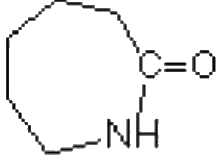
\includegraphics[width=1.5cm]{images_crop_de11/p3_cau5_caprolactam.png}
\end{center}
Một loại tơ capron có khối lượng phân tử là 14 916 amu. Số đơn vị mắt xích có trong phân tử loại tơ sợi này là bao nhiêu?
\par\noindent\textbf{Đáp số:} \textbf{\color{red}132}
\loigiai{
Trùng hợp mở vòng caprolactam tạo tơ capron có mắt xích là \ce{[-NH-(CH2)5-CO-]} ($M = 113\text{ amu}$).\\
Số đơn vị mắt xích là:
$$n = \frac{14916}{113} = 132.$$
\textbf{Đáp số: 132.}}
\end{ex}

\begin{ex}
Polymer A trong suốt, được dùng làm hộp đựng thực phẩm, đồ chơi trẻ em, vỏ đĩa CD, DVD,\dots{} Trong công nghiệp sản xuất chất dẻo, polymer A được điều chế theo sơ đồ:
\begin{center}
	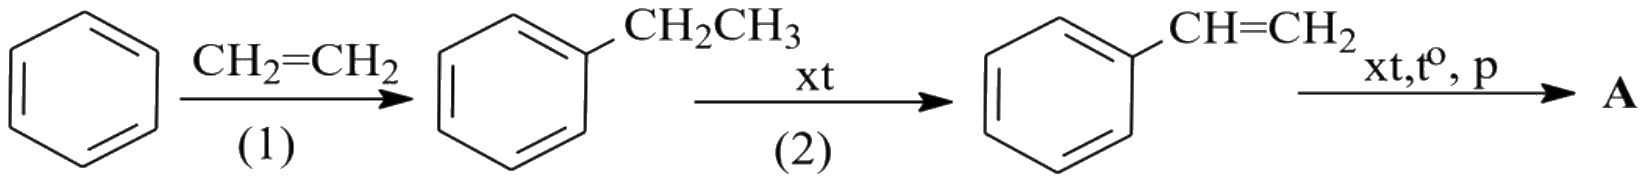
\includegraphics[width=10.5cm]{images_crop_de11/p3_cau6_scheme.png}
\end{center}
Từ $100\text{ kg}$ benzene và $32\text{ m}^3$ ethylene (ở 25 $^\circ\text{C}$, 1 bar), với hiệu suất mỗi quá trình (1), (2), (3) lần lượt là 60\%, 55\% và 60\%, hãy tính khối lượng polymer A thu được theo đơn vị kg (kết quả làm tròn đến chữ số hàng phần mười).
\par\noindent\textbf{Đáp số:} \textbf{\color{red}26,4}
\loigiai{
Tính số mol các chất tham gia:
$$n_{\text{benzene}} = \frac{100}{78} \approx 1{,}282\text{ kmol.}$$
Ở $25\ ^\circ\text{C}$, $1\text{ bar}$ ($V_m = 24{,}79\text{ m}^3/\text{kmol}$):
$$n_{\text{ethylene}} = \frac{32}{24{,}79} \approx 1{,}291\text{ kmol.}$$
Vì $n_{\text{benzene}} < n_{\text{ethylene}}$ nên lượng sản phẩm tính theo benzene.\\
Polymer A là polystyrene \ce{[-CH(C6H5)-CH2-]_n} ($M = 104\text{ kg/kmol}$).\\
Hiệu suất tổng của 3 giai đoạn:
$$H_{\text{tổng}} = 60\% \times 55\% \times 60\% = 0{,}60 \times 0{,}55 \times 0{,}60 = 0{,}198 = 19{,}8\%.$$
Khối lượng polymer A thu được là:
$$m_A = 1{,}282 \times 104 \times 19{,}8\% \approx 26{,}4\text{ kg.}$$
\textbf{Đáp số: 26,4.}}
\end{ex}


\Closesolutionfile{ans}

\vspace{0.5cm}
\begin{center}
	\textbf{\Large\color{mainGreen}BẢNG TỔNG HỢP ĐÁP ÁN ĐỀ SỐ 11}
\end{center}

\vspace{0.2cm}
\noindent\textbf{\color{mainGreen}PHẦN I: TRẮC NGHIỆM NHIỀU PHƯƠNG ÁN LỰA CHỌN}
\begin{center}
\renewcommand{\arraystretch}{1.2}
\begin{tabular}{|c|c|c|c|c|c|c|c|c|c|c|c|c|c|c|c|c|c|}
\hline
\textbf{1} & \textbf{2} & \textbf{3} & \textbf{4} & \textbf{5} & \textbf{6} & \textbf{7} & \textbf{8} & \textbf{9} & \textbf{10} & \textbf{11} & \textbf{12} & \textbf{13} & \textbf{14} & \textbf{15} & \textbf{16} & \textbf{17} & \textbf{18} \\ \hline
\textbf{\color{red}D} & \textbf{\color{red}D} & \textbf{\color{red}A} & \textbf{\color{red}B} & \textbf{\color{red}C} & \textbf{\color{red}D} & \textbf{\color{red}A} & \textbf{\color{red}B} & \textbf{\color{red}A} & \textbf{\color{red}A} & \textbf{\color{red}D} & \textbf{\color{red}A} & \textbf{\color{red}A} & \textbf{\color{red}D} & \textbf{\color{red}A} & \textbf{\color{red}A} & \textbf{\color{red}C} & \textbf{\color{red}D} \\ \hline
\end{tabular}
\end{center}

\vspace{0.3cm}
\noindent\textbf{\color{mainGreen}PHẦN II: TRẮC NGHIỆM ĐÚNG SAI}
\begin{center}
\renewcommand{\arraystretch}{1.2}
\begin{tabular}{|c|c|c|c|c|}
\hline
\textbf{Câu} & \textbf{Lệnh hỏi a} & \textbf{Lệnh hỏi b} & \textbf{Lệnh hỏi c} & \textbf{Lệnh hỏi d} \\ \hline
\textbf{1} & \textbf{S} & \textbf{\color{red}Đ} & \textbf{\color{red}Đ} & \textbf{\color{red}Đ} \\ \hline
\textbf{2} & \textbf{S} & \textbf{\color{red}Đ} & \textbf{\color{red}Đ} & \textbf{\color{red}Đ} \\ \hline
\textbf{3} & \textbf{\color{red}Đ} & \textbf{\color{red}Đ} & \textbf{\color{red}Đ} & \textbf{S} \\ \hline
\textbf{4} & \textbf{\color{red}Đ} & \textbf{S} & \textbf{S} & \textbf{\color{red}Đ} \\ \hline
\end{tabular}
\end{center}

\vspace{0.3cm}
\noindent\textbf{\color{mainGreen}PHẦN III: TRẢ LỜI NGẮN}
\begin{center}
\renewcommand{\arraystretch}{1.2}
\begin{tabular}{|c|c|c|c|c|c|}
\hline
\textbf{Câu 1} & \textbf{Câu 2} & \textbf{Câu 3} & \textbf{Câu 4} & \textbf{Câu 5} & \textbf{Câu 6} \\ \hline
\textbf{\color{red}4} & \textbf{\color{red}3} & \textbf{\color{red}2000} & \textbf{\color{red}6} & \textbf{\color{red}132} & \textbf{\color{red}26,4} \\ \hline
\end{tabular}
\end{center}

\end{document}
